\chapter{KI-basiertes Greifen}
\label{ch:kigreifen}
% Verantwortlich: Person 4 (Jeremy Zid).
% Entwurf 2026-10-30 aus seinen Unterlagen in code/m4_behavior_cloning/ (Requierments/requierments.md,
% Dokumentation/*.md, Berichte/*). Darf übernommen oder frei umgeschrieben werden.

Modul~4 greift das Bauteil nicht über eine programmierte Bahn, sondern mit einer gelernten
Policy (\cref{sec:ki-greifen-grundlagen}). Eine Diffusion Policy erhält in jedem Takt die
Bilder einer Kamera am Greifer und der Kamera über dem Arbeitsbereich sowie den Zustand des
Roboters und gibt die nächsten Gelenk-Sollwerte und den Greiferbefehl aus. Gelernt wird aus
Demonstrationen, die der Roboter selbst fährt (\ac{bc}, \cref{sec:bc-grundlagen}). Das
Modul ist eine Alternative zum klassischen Greifen von Modul~2 und für den automatischen
Ablauf nicht erforderlich.

% ------------------------------------------------------------------------------
\section{Aufgabe und Abgrenzung}
\label{sec:m4-aufgabe}

Im Ablauf übernimmt Modul~4 den Zustand PICK (\cref{tab:zustaende}). Die Policy startet in
einer festen Ausgangsstellung, sucht das Bauteil in den Kamerabildern, greift es und fährt es
an einen Übergabepunkt etwa \SI{9}{\centi\metre} über der Prüfvorrichtung. Dort endet ihre
Fahrt mit dem Bauteil im Greifer. Das Ablegen auf der Prüfvorrichtung (PLACE\_INSPECT) und alle
weiteren Bewegungen führt wieder Modul~2 aus. Die Pose aus der Objekterkennung wird an Modul~4
übergeben, aber nur protokolliert; die Policy bestimmt die Lage des Bauteils selbst aus den
Bildern.

Die gelernte Fahrt besteht aus sechs Abschnitten, die beim Aufzeichnen aus geteachten Punkten
geplant werden:
\begin{enumerate}
  \item eine Ausgangsstellung, in der der Arm das Bild der Draufsichtkamera freigibt,
  \item eine Anflugposition \SI{10}{\centi\metre} über der Vorgreifposition (\ac{ptp}),
  \item die Vorgreifposition \SI{5}{\centi\metre} über dem Greifpunkt (\ac{lin}),
  \item den Greifpunkt, an dem der Greifer schließt (\ac{lin}),
  \item die Rückkehr zur Vorgreifposition (\ac{lin}) und
  \item den Übergabepunkt über der Prüfvorrichtung (\ac{ptp}).
\end{enumerate}
Zwischen den Abschnitten wird überschliffen, damit der Arm an den Durchfahrpunkten nicht
anhält.

Der Greifer lässt sich über die Programmierschnittstelle nur öffnen und schließen; eine
Rückmeldung der Backenstellung gibt es nicht. Der Greiferzustand geht deshalb als binärer
Befehl in Zustand und Aktion ein. Nach jedem Greiferbefehl wartet die Bahn eine feste
Totzeit von \SI{0.5}{\second}, damit der Arm erst anhebt, wenn die Backen geschlossen sind.

\todo[inline]{Jeremy: Totzeit des Greifers (\SI{0.5}{\second}) an der Anlage messen
(Video) und hier bestätigen.}

% ------------------------------------------------------------------------------
\section{Hardware und Software}
\label{sec:m4-hardware}

\Cref{tab:m4-hardware} fasst die von Modul~4 genutzte Hardware zusammen. Roboter und Greifer
sind dieselben wie in Modul~2 (\cref{tab:hardware}).

\begin{table}[htbp]
  \centering
  \caption{Hardware und Software von Modul~4}
  \label{tab:m4-hardware}
  \begin{tabularx}{\textwidth}{@{}l X@{}}
    \toprule
    Komponente & Ausführung \\
    \midrule
    Handgelenkkamera & Daheng VEN-161-61U3C, Sony IMX296, $1440 \times 1080$~Pixel, Global
                       Shutter, bis \SI{61}{fps}, \ac{usb}3 Vision \\
    Objektiv & Fischauge, Brennweite \SI{1.85}{\milli\metre} \\
    Szenenkamera & Draufsichtkamera von Modul~1 (\cref{ch:objekterkennung}) \\
    Trainingsrechner & NVIDIA GeForce RTX 5070 Ti, \SI{16}{\giga\byte} Grafikspeicher \\
    Software & Python~3.12, PyTorch~2.11, LeRobot~0.6.1~\cite{lerobot}, NeuraPy 5.0.8 \\
    \bottomrule
  \end{tabularx}
\end{table}

Die Handgelenkkamera sitzt am Greifer und bewegt sich mit dem Arm. Ihre Lage zum Greifer ist
fest, sodass ein Verrutschen der Szene sie nicht betrifft. Ein Global-Shutter-Sensor belichtet
alle Pixel gleichzeitig; Bilder aus der Bewegung werden dadurch nicht verzerrt. Für das
Objektiv wurde ein Fischauge mit kurzer Brennweite gewählt, weil es den Arbeitsbereich vom
Anflug bis zum Greifpunkt scharf abbildet. Eine Unschärfe würde Information unwiederbringlich
verlieren, die starke, aber feste Verzeichnung des Fischauges lernt das Netz dagegen mit. Die
Kamera wird nicht über die übliche Videoschnittstelle angesprochen, sondern über das
Software-Paket des Herstellers (Galaxy SDK). Beide Kameras müssen direkt an den
\ac{usb}-3-Anschlüssen des Rechners hängen; über einen Verteiler erreichten sie in einem Test
nur 23 bis \SI{30}{fps}.

Das Training läuft vollständig lokal. Die Daten werden nicht in einen Cloud-Dienst
hochgeladen, und ein Datensatz kann zum Training auf einen anderen Rechner kopiert werden.

\begin{figure}[htbp]
  \centering
  \missingfigure[figwidth=0.9\textwidth]{Foto der Handgelenkkamera mit Fischaugenobjektiv am
  Greifer (Seitenansicht, Halterung und Kabelführung erkennbar).}
  \caption{Handgelenkkamera am Greifer}
  \label{fig:m4-kamera}
\end{figure}

% ------------------------------------------------------------------------------
\section{Beobachtung und Aktion}
\label{sec:m4-zustand}

Aufzeichnung und Ausführung laufen mit einem festen Takt von \SI{15}{\hertz}. In jedem Takt
wird eine Beobachtung gebildet und eine Aktion ausgeführt (\cref{tab:m4-zustand}).

\begin{table}[htbp]
  \centering
  \caption{Beobachtung und Aktion der Policy}
  \label{tab:m4-zustand}
  \begin{tabularx}{\textwidth}{@{}l l X@{}}
    \toprule
    Größe & Werte & Inhalt \\
    \midrule
    Zustand & 14 & sechs Gelenkwinkel in rad, \ac{tcp}-Position in m, \ac{tcp}-Orientierung als
                     Quaternion, Greiferbefehl (0 = offen, 1 = geschlossen) \\
    Bilder & 2 & Handgelenk- und Szenenkamera, je $240 \times 320$~Pixel, RGB \\
    Aktion & 7 & sechs Gelenkwinkel für den nächsten Takt (absolut), Greiferbefehl
                 (Schwelle 0,5) \\
    \bottomrule
  \end{tabularx}
\end{table}

Die Aktion ist eine absolute Gelenkstellung, nicht eine Änderung. Weil der Takt fest ist,
steckt die Geschwindigkeit des Roboters im Abstand zweier aufeinanderfolgender Aktionen. Die
Policy lernt also auch das Tempo der Aufzeichnung und fährt bei der Ausführung genauso
schnell. Deshalb müssen Takt, Bildgröße, Kameras, Geschwindigkeitsvorgaben und der Override
der Steuerung bei Aufzeichnung und Ausführung übereinstimmen. Weicht einer dieser Werte ab,
bricht die Ausführung ab, bevor sich der Roboter bewegt.

Zwischen den \SI{15}{\hertz}-Takten interpoliert das Modul je drei Zwischenwerte und sendet
die Gelenk-Sollwerte mit \SI{60}{\hertz} an die Steuerung (Befehl \texttt{servo\_j}).

% ------------------------------------------------------------------------------
\section{Datenaufnahme mit eingespeistem Rauschen}
\label{sec:m4-daten}

Demonstrationen werden nicht von Hand vorgeführt. Ein Bediener teacht nur die Punkte der
Bahn, mit einem Gamepad oder durch Handführung. Die eigentliche Aufzeichnung fährt der
Roboter selbst: Ein Bahnplaner verbindet die Punkte mit \ac{ptp}- und \ac{lin}-Abschnitten
konstanter Geschwindigkeit und prägt der Bahn dabei gezielt Rauschen auf (\cref{fig:m4-aufnahme}).
Dadurch ist das Tempo in allen Demonstrationen gleich, und es entstehen keine Pausen durch
Zögern des Bedieners, die die Policy als \enquote{stehen bleiben} lernen würde.

\begin{figure}[htbp]
  \centering
  \begin{tikzpicture}[pap]
    \node[pap term] (s) {Start};
    \node[pap proc=72mm, below=of s] (teach) {Punkte der Bahn teachen\\(Gamepad oder Handführung)};
    \node[pap proc=72mm, below=of teach] (lage) {Objektlage herstellen\\(von Hand oder vom Roboter neu ausgelegt)};
    \node[pap proc=72mm, below=of lage] (plan) {Ideale Bahn planen, Rauschstärke der Episode ziehen};
    \node[pap proc=72mm, below=of plan] (noise) {Kartesisches Rauschen aufprägen (Trichter zum Greifpunkt),\\
      per \acs{ik} in Gelenkwinkel umrechnen};
    \node[pap dec, below=of noise] (koll) {Kollisionsfrei?};
    \node[pap proc=72mm, below=of koll] (fahrt) {Fahren mit \SI{60}{\hertz}, aufzeichnen mit \SI{15}{\hertz}:\\
      Ist-Zustand und Bilder, ideale Soll-Stellung};
    \node[pap dec, below=of fahrt] (ok) {Episode gültig?};
    \node[pap proc=72mm, below=of ok] (save) {Episode speichern};
    \node[pap proc=40mm, right=12mm of ok] (drop) {Episode verwerfen};
    \node[pap proc=72mm, below=of save] (back) {Bauteil zurücklegen oder neu auslegen};
    \draw[pap arr] (s) -- (teach);
    \draw[pap arr] (teach) -- (lage);
    \draw[pap arr] (lage) -- (plan);
    \draw[pap arr] (plan) -- (noise);
    \draw[pap arr] (noise) -- (koll);
    \draw[pap arr] (koll) -- node[pap lbl, right] {ja} (fahrt);
    \draw[pap arr] (koll.east) -| node[pap lbl, above, pos=0.25] {nein} ($(noise.east)+(8mm,0)$)
      -- (noise.east);
    \draw[pap arr] (fahrt) -- (ok);
    \draw[pap arr] (ok) -- node[pap lbl, right] {ja} (save);
    \draw[pap arr] (ok) -- node[pap lbl, above] {nein} (drop);
    \draw[pap arr] (save) -- (back);
    \draw[pap arr] (drop) |- (back);
    \draw[pap arr] (back.west) -- ++(-14mm,0) |- (lage.west);
  \end{tikzpicture}
  \caption[Ablauf der automatischen Datenaufnahme]{Ablauf der automatischen Datenaufnahme.
  Eine Episode wird verworfen, wenn ein
  Schutzstopp auslöst, der Arm der Soll-Bahn zu weit hinterherläuft oder Kamerabild und
  Roboterzustand zeitlich nicht zusammenpassen.}
  \label{fig:m4-aufnahme}
\end{figure}

\subsection{Rauschen und asymmetrische Datenpaare}

Würde der Roboter immer genau die ideale Bahn fahren, enthielte der Datensatz kein einziges
Beispiel dafür, wie man von einer Abweichung zurückfindet (\cref{sec:bc-grundlagen}). Das
Modul folgt deshalb dem Gedanken von DART~\cite{laskey2017}: Während der Fahrt wird die Bahn
kartesisch ausgelenkt, und zwar mit einem Ornstein-Uhlenbeck-Prozess (\cref{eq:ou}) mit einer
Zeitkonstante von \SI{0.8}{\second}. Die Auslenkung ändert sich dadurch langsam und sieht
im Bild wie ein Schlingern aus, nicht wie ein Zittern. Die größte Amplitude liegt bei
\SI{15}{\milli\metre} in der Position und \SI{0.05}{rad} in der Drehung. Sie wurde
bewusst so groß gewählt, dass die Verschiebung im Kamerabild deutlich sichtbar ist.

Gespeichert werden die Daten asymmetrisch. Als Beobachtung dienen der tatsächliche, ausgelenkte
Zustand und die dabei aufgenommenen Bilder, als Aktion dagegen der nächste Punkt der
\emph{idealen} Bahn. Jedes Datenpaar zeigt der Policy also, wohin sie aus einer abweichenden
Lage steuern muss. Das Rauschen selbst taucht in den Aktionen nie auf und wird deshalb nicht
mitgelernt.

Kurz vor dem Greifpunkt muss die Bahn genau sein. Das Rauschen wird deshalb ab einem Abstand
von \SI{15}{\centi\metre} zum Greifpunkt gedämpft und ist ab \SI{2}{\centi\metre} ganz
abgeklungen (\cref{fig:m4-trichter}). Nach unten, zum Tisch hin, ist die Auslenkung
zusätzlich begrenzt. Die Rauschstärke wird für jede Episode zufällig zwischen null und der
vollen Amplitude gezogen. So enthält der Datensatz sowohl ruhige Fahrten nahe der Idealbahn als
auch Fahrten mit großen Korrekturen.

\begin{figure}[htbp]
  \centering
  \begin{tikzpicture}[font=\small, x=1cm, y=1cm]
    % Rauschkorridor
    \fill[blue!8] (0,1) -- (6.5,1) -- (9.3,0) -- (6.5,-1) -- (0,-1) -- cycle;
    \draw[blue!40, densely dashed] (0,1) -- (6.5,1) -- (9.3,0);
    \draw[blue!40, densely dashed] (0,-1) -- (6.5,-1) -- (9.3,0);
    % ideale Bahn
    \draw[thick] (0,0) -- (10,0);
    \fill (0,0) circle (2pt) node[left] {Start};
    \fill (10,0) circle (2pt) node[right] {Greifpunkt};
    % gefahrene Bahn
    \draw[red!70!black, thick] plot[smooth, tension=0.7] coordinates
      {(0,0) (0.9,0.45) (1.8,0.75) (2.7,0.3) (3.6,-0.5) (4.5,-0.8) (5.4,-0.2) (6.3,0.55)
       (7.2,0.4) (8.1,-0.15) (8.8,0.05) (9.4,0) (10,0)};
    % Korrekturpfeile
    \foreach \x/\y in {1.8/0.75, 4.5/-0.8, 6.3/0.55} {
      \draw[-{Stealth[length=1.6mm]}, green!50!black, thick] (\x,\y) -- (\x+0.7,0.04*\y);
    }
    % Maße
    \draw[{Stealth[length=1.4mm]}-{Stealth[length=1.4mm]}] (0.3,-1) -- (0.3,1)
      node[above, font=\scriptsize] {Amplitude};
    \draw[densely dotted] (6.5,-1.1) -- (6.5,-1.5);
    \draw[densely dotted] (9.3,-0.1) -- (9.3,-1.5);
    \draw[densely dotted] (10,-0.1) -- (10,-1.5);
    \draw[{Stealth[length=1.4mm]}-{Stealth[length=1.4mm]}] (6.5,-1.4) -- node[below, font=\scriptsize] {\SI{15}{\centi\metre}} (10,-1.4);
    \node[font=\scriptsize, anchor=north] at (9.65,-1.6) {\SI{2}{\centi\metre}};
    % Legende
    \begin{scope}[shift={(0,-2.4)}, font=\scriptsize]
      \draw[thick] (0,0) -- (0.6,0); \node[anchor=west] at (0.7,0) {ideale Bahn (Aktion)};
      \draw[red!70!black, thick] (4.0,0) -- (4.6,0); \node[anchor=west] at (4.7,0) {gefahrene Bahn (Beobachtung)};
      \draw[-{Stealth[length=1.6mm]}, green!50!black, thick] (9.3,0) -- (9.9,0); \node[anchor=west] at (10.0,0) {gelernte Korrektur};
    \end{scope}
  \end{tikzpicture}
  \caption[Rauschkorridor um die ideale Bahn]{Rauschkorridor um die ideale Bahn
  (schematisch). Die Auslenkung ist bis
  \SI{15}{\centi\metre} vor dem Greifpunkt voll wirksam, wird danach gedämpft und ist
  \SI{2}{\centi\metre} vor dem Greifpunkt null. Aus der Paarung von ausgelenktem Zustand und
  idealer Soll-Stellung lernt die Policy, zur Bahn zurückzusteuern.}
  \label{fig:m4-trichter}
\end{figure}

\subsection{Umrechnung und Kollisionsprüfung}

Das Rauschen ist kartesisch festgelegt, weil sich nur so eine Grenze in eine feste Richtung,
etwa zum Tisch hin, sicher einhalten lässt. Die verrauschte Bahn wird vor der Fahrt mit der
inversen Kinematik der Robotersteuerung in Gelenkwinkel umgerechnet. Als Startwert dient
jeweils die Lösung des vorherigen Schritts, sodass die Lösung nicht zwischen verschiedenen
Armstellungen springt. Ein Vortest an drei realen Posen ergab, dass alle Punkte im Korridor
von \SI{\pm 20}{\milli\metre} erreichbar sind und die Bahn weit von singulären Stellungen
entfernt liegt.

Anschließend wird die gesamte Bahn gegen ein einfaches Kollisionsmodell geprüft. Tisch und
feste Hindernisse sind als Quader beschrieben, und für mehrere Punkte entlang des Arms wird
der Abstand zu diesen Quadern berechnet. Unterschreitet ein Punkt einen Sicherheitsabstand von
\SI{3}{\centi\metre}, wird das Rauschen neu gezogen.

\subsection{Objektlagen}

Damit die Policy das Bauteil an beliebigen Stellen findet, muss der Datensatz viele
verschiedene Objektlagen enthalten. Für jede Lage werden die Greifpunkte nachgeteacht. Um
diesen Aufwand zu verringern, legt der Roboter das Bauteil nach jeder Episode selbst wieder ab:
entweder an derselben Stelle, um die Bahn mit neuem Rauschen erneut aufzuzeichnen, oder an
einer neuen, zufällig gezogenen Lage innerhalb des Arbeitsbereichs mit einer Drehung bis
\ang{\pm 45}. Die neue Lage ist dann genau bekannt und wird als Zahl in den Metadaten der
Episode gespeichert. Diese Fahrten werden nicht aufgezeichnet.

Als Richtgröße für den Umfang werden einige Dutzend bis wenige Hundert Demonstrationen
angesetzt. Die tatsächlich benötigte Anzahl ergibt sich erst aus den Trainingsergebnissen.

% ------------------------------------------------------------------------------
\section{Modell und Training}
\label{sec:m4-training}

Eingesetzt wird die faltungsbasierte Diffusion Policy~\cite{chi2024} aus LeRobot
(\cref{sec:diffusion-policy}). Jede Kamera hat einen eigenen Bildkodierer, ein ResNet18 mit
vortrainierten ImageNet-Gewichten~\cite{he2016}. Seine Merkmale werden mit dem Zustand der
letzten beiden Takte zusammengefasst und an ein eindimensionales U-Net übergeben, das eine
Folge von 16 Aktionen entrauscht. \Cref{tab:m4-hyper} listet die wichtigsten Einstellungen.

\begin{table}[htbp]
  \centering
  \caption{Einstellungen der Diffusion Policy}
  \label{tab:m4-hyper}
  \begin{tabularx}{\textwidth}{@{}l X@{}}
    \toprule
    Parameter & Wert \\
    \midrule
    Bildkodierer & ResNet18 je Kamera, ImageNet-Gewichte \\
    U-Net-Kanäle & 256, 512, 1024 \\
    Parameter gesamt & \num{89.5} Millionen \\
    Beobachtungen & 2 Takte \\
    Vorhersagehorizont & 16 Aktionen, davon 8 nutzbar \\
    Entrauschen & 100 Schritte im Training, 10 Schritte (DDIM) bei der Ausführung \\
    Vorhersageziel & Aktionsfolge direkt (nicht das Rauschen) \\
    Bildaugmentierung & zufälliger Ausschnitt \SI{90}{\percent} \\
    Optimierer & AdamW, Lernrate $10^{-4}$, Cosinus-Verlauf, gleitender Mittelwert der
                 Gewichte (0,999) \\
    Batchgröße, Schritte & 64, \num{60000} (Vorgabe) \\
    \bottomrule
  \end{tabularx}
\end{table}

Die Größe des U-Nets ist kleiner als die Vorgabe von LeRobot. So passt das Training in die
\SI{16}{\giga\byte} der Grafikkarte, und die Vorhersage bleibt auf kleineren Rechnern
ausführbar. Auf der RTX 5070 Ti dauert ein Trainingsschritt mit Batchgröße 64 etwa
\SI{0.21}{\second}; die vorgegebenen \num{60000} Schritte dauern damit rund
\SI{3.5}{\hour}.

Für das Vorhersageziel wurde die Aktionsfolge selbst gewählt statt des enthaltenen
Rauschens. Bei nur zehn Entrauschungsschritten erzeugte die Rauschvorhersage in einem
Vergleich gezackte Aktionsfolgen mit Sprüngen von \num{0.10} bis \SI{0.12}{rad}, während
die Sprünge in den Trainingsdaten bei \SI{0.015}{rad} lagen. Mit der direkten Vorhersage
der Folge entsprechen die Sprünge denen der Trainingsdaten.

% ------------------------------------------------------------------------------
\section{Ausführung}
\label{sec:m4-inferenz}

Vor jeder Fahrt wird der Greifer in seinen Ausgangszustand gebracht, und der Arm fährt die
Ausgangsstellung der Aufzeichnung an. Danach läuft der Takt aus \cref{fig:m4-takt}.

\begin{figure}[htbp]
  \centering
  \begin{tikzpicture}[pap]
    \node[pap term] (s) {Takt $t$ (\SI{15}{\hertz})};
    \node[pap proc=80mm, below=of s] (obs) {Beobachtung bilden: beide Kamerabilder und Zustand der
      letzten zwei Takte};
    \node[pap proc=80mm, below=of obs] (pol) {alle 2 Takte: neue Aktionsfolge vorhersagen
      (eigener Thread, $\approx$\SI{77}{\milli\second})};
    \node[pap proc=80mm, below=of pol] (mix) {alle Vorhersagen für Takt $t$ mitteln};
    \node[pap proc=80mm, below=of mix] (lim) {Änderung auf \SI{0.8}{rad/s} begrenzen,\\
      Abstand Soll--Ist und Arbeitsraum prüfen};
    \node[pap proc=80mm, below=of lim] (send) {4 interpolierte Sollwerte mit \SI{60}{\hertz} senden,\\
      jeden Sollwert auf \SI{1.0}{rad/s} prüfen, Greiferbefehl bei Wechsel};
    \node[pap dec, below=of send] (end) {Übergabepunkt\\erreicht?};
    \node[pap good, below=of end] (done) {Übergabe an Modul~2};
    \node[pap bad, right=12mm of lim] (stop) {Stopp};
    \draw[pap arr] (s) -- (obs);
    \draw[pap arr] (obs) -- (pol);
    \draw[pap arr] (pol) -- (mix);
    \draw[pap arr] (mix) -- (lim);
    \draw[pap arr] (lim) -- (send);
    \draw[pap arr] (send) -- (end);
    \draw[pap arr] (end) -- node[pap lbl, right] {ja} (done);
    \draw[pap arr] (end.west) -| node[pap lbl, above, pos=0.25] {nein} ($(send.west)+(-8mm,0)$)
      |- (s.west);
    \draw[pap arr] (lim.east) -- node[pap lbl, above] {verletzt} (stop);
    \draw[pap arr] (send.east) -| (stop.south);
  \end{tikzpicture}
  \caption{Ablauf eines Takts bei der Ausführung der Policy}
  \label{fig:m4-takt}
\end{figure}

Eine Vorhersage mit zehn Entrauschungsschritten dauert auf der RTX 5070 Ti etwa
\SI{77}{\milli\second} und damit länger als ein Takt von \SI{67}{\milli\second}. Sie läuft
deshalb in einem eigenen Thread. Der Sollwertstrom an den Roboter läuft ungestört weiter,
und jede Vorhersage wird dem Takt zugeordnet, aus dem ihre Beobachtung stammt. Teile einer
Vorhersage, die bei ihrem Eintreffen schon vorbei sind, verfallen. Reicht keine Vorhersage mehr
bis zum aktuellen Takt, wird die Fahrt beendet.

Weil alle zwei Takte neu vorhergesagt wird und jede Vorhersage acht nutzbare Aktionen hat,
liegen für einen Takt bis zu vier Vorhersagen vor. Ausgeführt wird ihr Mittelwert, wie von
Zhao et al.\ vorgeschlagen~\cite{zhao2023}. Das glättet den Übergang, wenn eine neue Vorhersage
eintrifft.

Die Fahrt gilt als beendet, wenn die Gelenke fünf Takte lang höchstens \SI{0.02}{rad}
von der Endstellung der Aufzeichnung entfernt sind und der Greifer geschlossen ist. Die
Stellung allein reicht nicht, weil der Arm auf dem Hin- und Rückweg dieselben Stellungen
durchfahren kann und sich dann nur der Greiferzustand unterscheidet.

% ------------------------------------------------------------------------------
\section{Sicherheitsmaßnahmen}
\label{sec:m4-sicherheit}

Eine gelernte Policy kann unerwartete Sollwerte ausgeben. Zusätzlich zu den Schutzfunktionen
des \ac{cobot}s prüft Modul~4 deshalb jeden Befehl, bevor er gesendet wird:

\begin{description}
  \item[Weiche Begrenzung] Die Änderung der Sollstellung je Takt wird auf eine
    Gelenkgeschwindigkeit von \SI{0.8}{rad/s} begrenzt, die Richtung bleibt erhalten.
  \item[Harte Grenze] Jeder einzelne \SI{60}{\hertz}-Sollwert wird verworfen, wenn er nicht
    endlich ist, außerhalb der Achsgrenzen liegt oder eine Gelenkgeschwindigkeit über
    \SI{1.0}{rad/s} erfordert. Liegt die Sollstellung mehr als \SI{0.35}{rad} von der
    gemessenen Stellung entfernt, wird ebenfalls nichts gesendet. In beiden Fällen stoppt
    der Roboter.
  \item[Arbeitsraumüberwachung] Ein eigener Thread prüft laufend die Lage von Werkzeug und Arm
    gegen dasselbe Kollisionsmodell wie bei der Aufnahme und stoppt bei einer Verletzung.
  \item[Schleppfehler] Bei der Aufnahme wird abgebrochen, wenn der Arm vier Takte lang mehr als
    \SI{0.30}{rad} hinter der Sollstellung liegt.
  \item[Freigabe] Fahrten am realen Roboter erfordern eine ausdrückliche Bestätigung.
\end{description}

Der Software-Stopp hält den Arm nach Messungen an der Anlage innerhalb von
\SI{96}{\milli\second} an. Er ersetzt keinen Not-Halt; der Hardware-Not-Halt bleibt bei allen
Fahrten in Reichweite.

% ------------------------------------------------------------------------------
\section{Ausführungsart an der Anlage}
\label{sec:m4-zittern}

In der virtuellen Maschine (\ac{vm}) der Steuerung lief die Ausführung über \texttt{servo\_j}
mit \SI{60}{\hertz} ruhig. Am realen Roboter zitterte der Arm dagegen deutlich. Die Steuerung
fährt jeden Sollwert an und wartet dann auf den nächsten, sodass bei \SI{60}{\hertz} eine
treppenförmige Bewegung entsteht. Sie regt Arm und Aufbau bei \SIrange{7}{8}{\hertz} an
(\cref{fig:m4-spektrum}). Gemessen wurde die Schwingung mit dem Beschleunigungssensor eines
Smartphones am Unterarm des Roboters.

\begin{figure}[htbp]
  \centering
  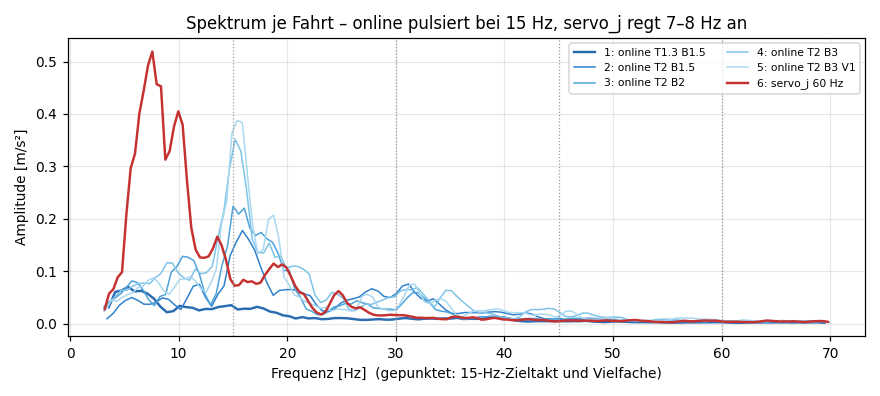
\includegraphics[width=\textwidth]{m4/03_handy_spektrum.png}
  \caption[Spektrum der Beschleunigung am Unterarm je Ausführungsart]{Spektrum der
  Beschleunigung am Unterarm je Fahrt. Rot:
  \texttt{servo\_j} mit \SI{60}{\hertz}; blau: Varianten mit Interpolation in der Steuerung
  (\texttt{movelinear\_online}). Quelle: Unterlagen Modul~4.}
  \label{fig:m4-spektrum}
\end{figure}

Untersucht wurden zwei Abhilfen. Lässt man die Steuerung selbst zwischen Zielpunkten
interpolieren (\texttt{movelinear\_online}), sinkt das Zittern deutlich, der Arm weicht aber
in Kurven und Drehungen um bis zu \SI{49}{\milli\metre} von der geplanten Bahn ab und läuft
bis zu \SI{0.79}{rad} hinterher. Das widerspricht den Datenpaaren aus
\cref{sec:m4-daten}, bei denen Zustand und Sollstellung zueinander passen müssen. Wird
dagegen \texttt{servo\_j} beibehalten und der Override der Steuerung auf \num{0.5} gesetzt,
führt die Steuerung die Sollwerte weicher nach. In einer Messreihe am Roboter lag die
Schwingung damit bei
\SIrange{0.19}{0.20}{\metre\per\second\squared} statt \SI{1.74}{\metre\per\second\squared},
also auf dem Niveau eines Programms am Bedienhandgerät des Herstellers
(\SIrange{0.16}{0.18}{\metre\per\second\squared}, \cref{fig:m4-h1}). Die Bahn wich um
höchstens \SI{1.2}{\milli\metre} ab, und die Fahrzeit blieb mit \SI{11.6}{\second} gleich.
Für Aufnahme und Ausführung wurde deshalb \texttt{servo\_j} mit Override \num{0.5} festgelegt.

\begin{figure}[htbp]
  \centering
  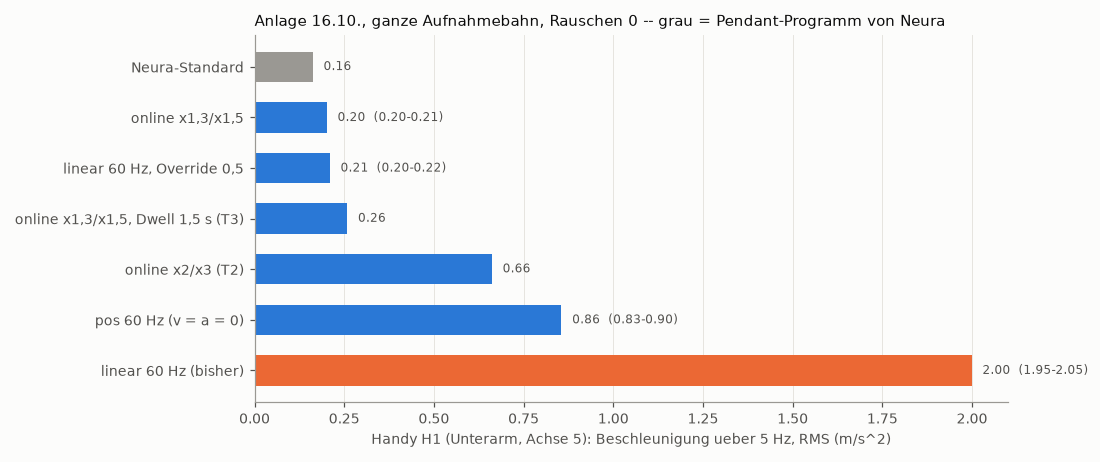
\includegraphics[width=\textwidth]{m4/13_labortag16_h1.png}
  \caption[Schwingung am Unterarm je Ausführungsart]{Schwingung am Unterarm über die ganze
  Aufnahmebahn je Ausführungsart (Effektivwert
  der Beschleunigung oberhalb \SI{5}{\hertz}, ohne Rauschen). Grau: Programm
  am Bedienhandgerät als Vergleich. Quelle: Unterlagen Modul~4.}
  \label{fig:m4-h1}
\end{figure}

\todo[inline]{Jeremy: Override \num{0.5} mit dem Betreuer abstimmen (Sicherheitsthema) und
hier vermerken.}

% ------------------------------------------------------------------------------
\section{Einbindung in das Gesamtsystem}
\label{sec:m4-integration}

Modul~4 ist mit der Schnittstelle \texttt{Grasper} in das System eingebunden
(\cref{tab:modulschnittstellen}). Die Variante \texttt{BcGrasper} führt beim Greifen genau eine
Fahrt der Policy aus. Weil LeRobot~0.6.1 Python~3.12 voraussetzt und seine Abhängigkeiten
mit denen der Texterkennung von Modul~3 kollidieren, läuft die Policy in einer eigenen
Python-Umgebung als Unterprozess. Die Bedienoberfläche und die übrigen Module bleiben in ihrer
Umgebung.

Ein Greifvorgang mit Modul~4 läuft so ab:
\begin{enumerate}
  \item Die Objekterkennung gibt die Draufsichtkamera frei, damit Modul~4 sie als Szenenkamera
        öffnen kann. Die Robotersteuerung von Modul~2 trennt ihre Verbindung zur Steuerung.
  \item Der Unterprozess startet die Policy und fährt den Roboter über eine eigene Verbindung.
        Bei Fahrten am realen Roboter wird die Freigabe aus dem Sicherheitsdialog des Ablaufs
        übernommen (\cref{sec:int-fehler}).
  \item Der Fortschritt wird aus der Ausgabe des Unterprozesses gelesen. Erreicht die Policy den
        Übergabepunkt nicht oder dauert die Fahrt länger als \SI{300}{\second}, gilt das Greifen
        als fehlgeschlagen, und der Ablauf geht in den Fehlerzustand.
  \item Für das Ablegen verbindet sich Modul~2 wieder, setzt Werkzeug, Override und
        Bewegungsprogramm auf seine eigenen Werte zurück und legt das Bauteil auf der
        Prüfvorrichtung ab.
\end{enumerate}

Dass immer nur eine Seite den Roboter und die Draufsichtkamera benutzt, regelt die
Bedienoberfläche (\cref{sec:int-gui}). Daneben enthält sie einen eigenen Reiter für Modul~4 mit
Systemcheck, Aufnahme, Training und Betrieb.

% ------------------------------------------------------------------------------
\section{Stand und Ergebnisse}
\label{sec:m4-ergebnisse}

Bisher wurde die Kette aus Aufnahme, Training und Ausführung in zwei Umgebungen erprobt: in
einer eigenen Simulation des Roboters und in der \ac{vm} der Neura-Steuerung. In beiden Fällen
lieferten die Kameras nur Platzhalterbilder ohne Bezug zur Szene. Die Policy konnte also nur
aus dem Zustand lernen; geprüft wurde die Kette, nicht die spätere Greifqualität.

\begin{table}[htbp]
  \centering
  \caption[Erprobung der Kette mit Platzhalterbildern]{Erprobung der Kette mit
  Platzhalterbildern. Erfolg: Greifer schließt
  höchstens \SI{10}{\milli\metre} neben dem Greifpunkt der Aufzeichnung, und die Fahrt endet
  höchstens \SI{10}{\milli\metre} neben dem Übergabepunkt. Werte als Median über die Fahrten.}
  \label{tab:m4-durchstich}
  \begin{tabularx}{\textwidth}{@{}X r r r r@{}}
    \toprule
    Umgebung (Datensatz) & Erfolg & Greifpunkt & Bahn p95 & Vorhersage \\
    \midrule
    Simulation (50 Episoden) & 10/10 & \SI{1.6}{\milli\metre} & \SI{4.0}{\milli\metre} & \SI{117}{\milli\second} \\
    \ac{vm} der Steuerung (30 Episoden) & 0/5 & -- & \SI{5.2}{\milli\metre} & \SI{85}{\milli\second} \\
    \bottomrule
  \end{tabularx}
\end{table}

In der Simulation führte die Policy die Aufgabe in allen zehn Fahrten selbst aus
(\cref{tab:m4-durchstich,fig:m4-rollouts}). In der \ac{vm} folgte sie der Bahn bis zur
Vorgreifposition, blieb dort aber in allen Fahrten stehen. An dieser Stelle endet in den Daten
eine \ac{ptp}-Fahrt im Stillstand, und die folgende \ac{lin}-Fahrt beginnt aus dem Stillstand.
Im Zustand sind \enquote{angekommen} und \enquote{losfahren} dort nicht zu unterscheiden, und
die Policy sagt \enquote{stehen bleiben} vorher. Daraufhin wurde der Bahnplaner so geändert,
dass er an der Vorgreifposition mit \SI{10}{\milli\metre} überschleift (\cref{sec:m4-aufgabe}).
Am Greifpunkt selbst bleibt ein Halt, weil der Arm dort für das Schließen des Greifers wartet.
Ob die Policy diesen Halt mit echten Bildern überwindet, ist noch offen.

\begin{figure}[htbp]
  \centering
  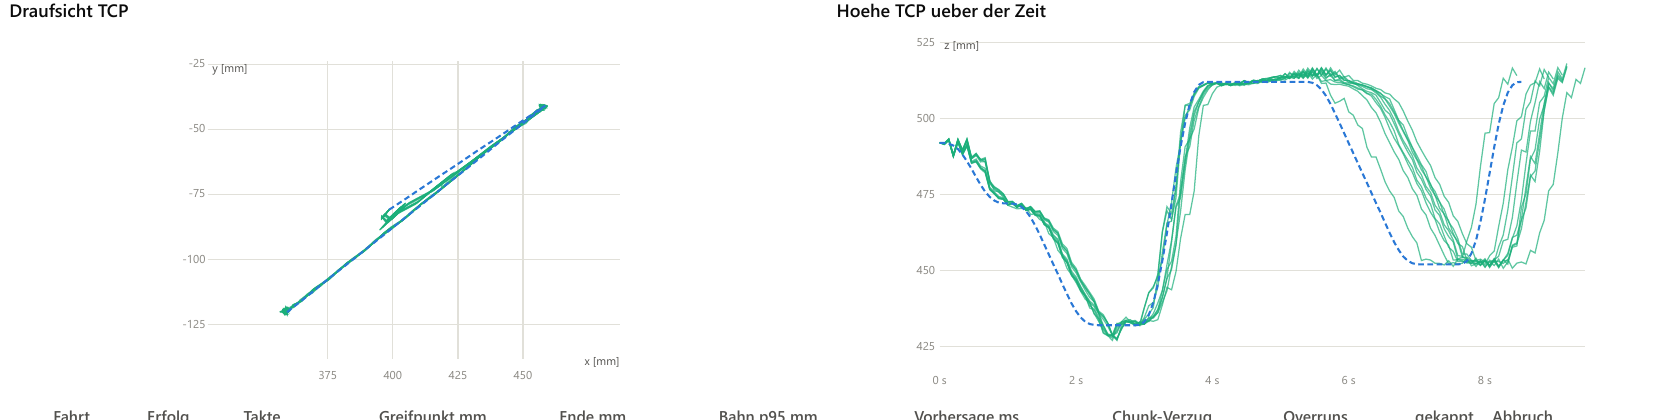
\includegraphics[width=\textwidth]{m4/durchstich_sim_rollouts.png}
  \caption[Zehn Fahrten der Policy in der Simulation]{Zehn Fahrten der Policy in der
  Simulation: Draufsicht (links) und Höhe des \ac{tcp}
  über der Zeit (rechts). Blau gestrichelt die ideale Bahn der Aufzeichnung, grün die
  Fahrten der Policy. Quelle: Unterlagen Modul~4.}
  \label{fig:m4-rollouts}
\end{figure}

Ob das eingespeiste Rauschen nützt, wurde vorab in einer Ersatzstudie ohne Bilder untersucht.
Dafür wurde mit derselben Planungs- und Rauschkette ein einfaches Netz trainiert und in einer
Simulation mit verschobenen Objektlagen und seitlichen Stößen von \SI{15}{\milli\metre}
geprüft (5 Trainingsläufe mit je 24 Objektlagen). \Cref{tab:m4-rauschstudie} zeigt das
Ergebnis. Ohne Rauschen gelang ein Drittel der Fahrten, mit Rauschen etwa neun von zehn. Die
gewählte Einstellung, eine je Episode zufällige Rauschstärke, war bei Stößen am besten und
erzeugte zugleich die ruhigsten Bewegungen. Da die Studie ohne Bilder und mit einem anderen
Netz arbeitet, lässt sich das Ergebnis nur der Tendenz nach auf die Anlage übertragen.

\begin{table}[htbp]
  \centering
  \caption[Ersatzstudie zum eingespeisten Rauschen]{Ersatzstudie zum eingespeisten Rauschen
  (ohne Bilder). Erfolg: Greifen
  weniger als \SI{5}{\milli\metre} neben dem Greifpunkt und Übergabe mit geschlossenem Greifer.}
  \label{tab:m4-rauschstudie}
  \begin{tabularx}{\textwidth}{@{}X r r r@{}}
    \toprule
    Rauschen & Erfolg ungestört & Erfolg mit Stößen & Greiffehler \\
    \midrule
    ohne & \SI{32}{\percent} & \SI{12}{\percent} & \SI{3.4}{\milli\metre} \\
    fest, \SI{15}{\milli\metre} / \ang{2.9} & \SI{90}{\percent} & \SI{92}{\percent} & \SI{0.6}{\milli\metre} \\
    je Episode zufällig, 0--\SI{15}{\milli\metre} / 0--\ang{2.9} & \SI{92}{\percent} & \SI{93}{\percent} & \SI{0.5}{\milli\metre} \\
    \bottomrule
  \end{tabularx}
\end{table}

Am realen Roboter sind Aufnahme und Kameras in Betrieb genommen. Sechs Aufnahme-Episoden mit
der endgültigen Ausführungsart, noch mit Platzhalterbildern und ohne Greiferansteuerung,
liefen ohne Abbruch; der Arm lag dabei höchstens
\SIrange{0.06}{0.10}{rad} hinter der Sollstellung, weit innerhalb der Grenzen aus
\cref{sec:m4-sicherheit}. Bei der ersten Aufnahme mit beiden echten Kameras wurden alle drei
Episoden verworfen, weil die Handgelenkkamera über einen \ac{usb}-Verteiler nur
\SI{23}{fps} lieferte und dadurch zu viele Bilder älter als \SI{30}{\milli\second} waren.
Direkt am Rechner erreicht die Kamera ihre volle Bildrate.

\begin{figure}[htbp]
  \centering
  \missingfigure[figwidth=0.9\textwidth]{Je ein Bild der Handgelenk- und der Szenenkamera aus
  einer echten Aufnahme in der Auflösung der Policy ($240 \times 320$~Pixel), z.\,B.\ kurz vor dem
  Greifen.}
  \caption{Beobachtung der Policy: Handgelenkkamera (links) und Szenenkamera (rechts)}
  \label{fig:m4-bilder}
\end{figure}

% ------------------------------------------------------------------------------
\section{Zwischenfazit}
\label{sec:m4-fazit}

Die Kette aus automatischer Aufnahme mit eingespeistem Rauschen, Training einer Diffusion
Policy und Ausführung mit Sicherheitsprüfungen ist umgesetzt und in den automatischen Ablauf
eingebunden. In der Simulation fährt die Policy die Aufgabe zuverlässig; in der \ac{vm} hat
die Erprobung eine Schwäche des Datendesigns an Haltepunkten gezeigt, die an der
Vorgreifposition im Bahnplaner behoben ist und am Greifpunkt noch beobachtet werden muss. Am realen Roboter wurde eine Ausführungsart gefunden, die so ruhig ist wie ein
Programm des Herstellers und die Bahn dabei genau einhält. Eine Aussage zur Greifqualität ist
erst nach dem Training mit echten Bildern möglich.

\todo[inline]{Jeremy: Zwischenfazit nach den Versuchen mit echtem Datensatz ergänzen.}
